
\documentclass[a4paper,12pt]{book}
\usepackage{natbib}
\usepackage[utf8]{inputenc}
\usepackage[T1]{fontenc}
%\usepackage[frenchb]{babel} % If you write in French
\usepackage[english]{babel} % If you write in English
\usepackage{a4wide}
\usepackage{graphicx}
\graphicspath{{figures/}}
%\usepackage{subfig}
%\usepackage{tikz}
%\usetikzlibrary{shapes,arrows}
%\usepackage{pgfplots}
%\pgfplotsset{compat=newest}
%\pgfplotsset{plot coordinates/math parser=false}
%\newlength\figureheight
%\newlength\figurewidth
%\pgfkeys{/pgf/number format/.cd,
%set decimal separator={,\!},
%1000 sep={\,},
%}
%\usepackage{ifthen}
%\usepackage{ifpdf}

%\ifpdf
%\usepackage[pdftex]{hyperref}
%\else
%\usepackage{hyperref}
%\fi
\usepackage[usenames,dvipsnames]{color}
\usepackage{hyperref}
\hypersetup{
	colorlinks=false, %set true if you want colored links
	linktoc=all,     %set to all if you want both sections and subsections linked
	linkcolor=blue,  %choose some color if you want links to stand out
	urlcolor=blue,
	linktocpage
}
\usepackage{makecell} % manage linebreak within a cell

\renewcommand{\baselinestretch}{1.05}
\usepackage{fancyhdr}
\pagestyle{fancy}
\fancyfoot{}
\fancyhead[LE,RO]{\bfseries\thepage}
\fancyhead[RE]{\bfseries\nouppercase{\leftmark}}
\fancyhead[LO]{\bfseries\nouppercase{\rightmark}}
\setlength{\headheight}{15pt}

\let\headruleORIG\headrule
\renewcommand{\headrule}{\color{black} \headruleORIG}
\renewcommand{\headrulewidth}{1.0pt}
\usepackage{colortbl}
\arrayrulecolor{black}
\fancypagestyle{plain}{
  \fancyhead{}
  \fancyfoot[C]{\thepage}
  \renewcommand{\headrulewidth}{0pt}
}

\makeatletter
\def\@textbottom{\vskip \z@ \@plus 1pt}
\let\@texttop\relax
\makeatother

\makeatletter
\def\cleardoublepage{\clearpage\if@twoside \ifodd\c@page\else%
  \hbox{}%
  \thispagestyle{empty}%
  \newpage%
  \if@twocolumn\hbox{}\newpage\fi\fi\fi}
\makeatother

\usepackage{amsthm}
\usepackage{amssymb,amsmath,bbm}
\usepackage{array}
\usepackage{bm}
\usepackage{multirow}
\usepackage[footnote]{acronym}

\usepackage{framed}
\usepackage{listings}
%\lstset{language=R,keywordstyle=\color{blue},basicstyle=\ttfamily,breaklines=true}
\lstset{ 
	language=R,                     % the language of the code
	basicstyle=\ttfamily, % the size of the fonts that are used for the code
	numbers=left,                   % where to put the line-numbers
	numberstyle=\color{Blue},  % the style that is used for the line-numbers
	stepnumber=1,                   % the step between two line-numbers. If it is 1, each line
	% will be numbered
	numbersep=5pt,                  % how far the line-numbers are from the code
	backgroundcolor=\color{white},  % choose the background color. You must add \usepackage{color}
	showspaces=false,               % show spaces adding particular underscores
	showstringspaces=false,         % underline spaces within strings
	showtabs=false,                 % show tabs within strings adding particular underscores
	frame=single,                   % adds a frame around the code
	rulecolor=\color{Gray},        % if not set, the frame-color may be changed on line-breaks within not-black text (e.g. commens (green here))
	tabsize=2,                      % sets default tabsize to 2 spaces
	captionpos=b,                   % sets the caption-position to bottom
	breaklines=true,                % sets automatic line breaking
	breakatwhitespace=false,        % sets if automatic breaks should only happen at whitespace
	keywordstyle=\color{RoyalBlue},      % keyword style
	commentstyle=\color{LimeGreen},   % comment style
	stringstyle=\color{ForestGreen},      % string literal style
	deletekeywords={max,factor,local},
	morekeywords={expe2df,runexpplan,writemodelparameterfile,setparametervalue,setfinalstep,setoutputframerate,setmodelpath,setsimulationid,setseed,addtoexperimentplan,paste0,readNamesXMLOutputs,xmlToDataFrame}
} 

\usepackage{datetime}

\begin{document}

%%%%%%%%%%%%%%%%%%
%%% First page %%%
%%%%%%%%%%%%%%%%%%

\begin{titlepage}
\begin{center}

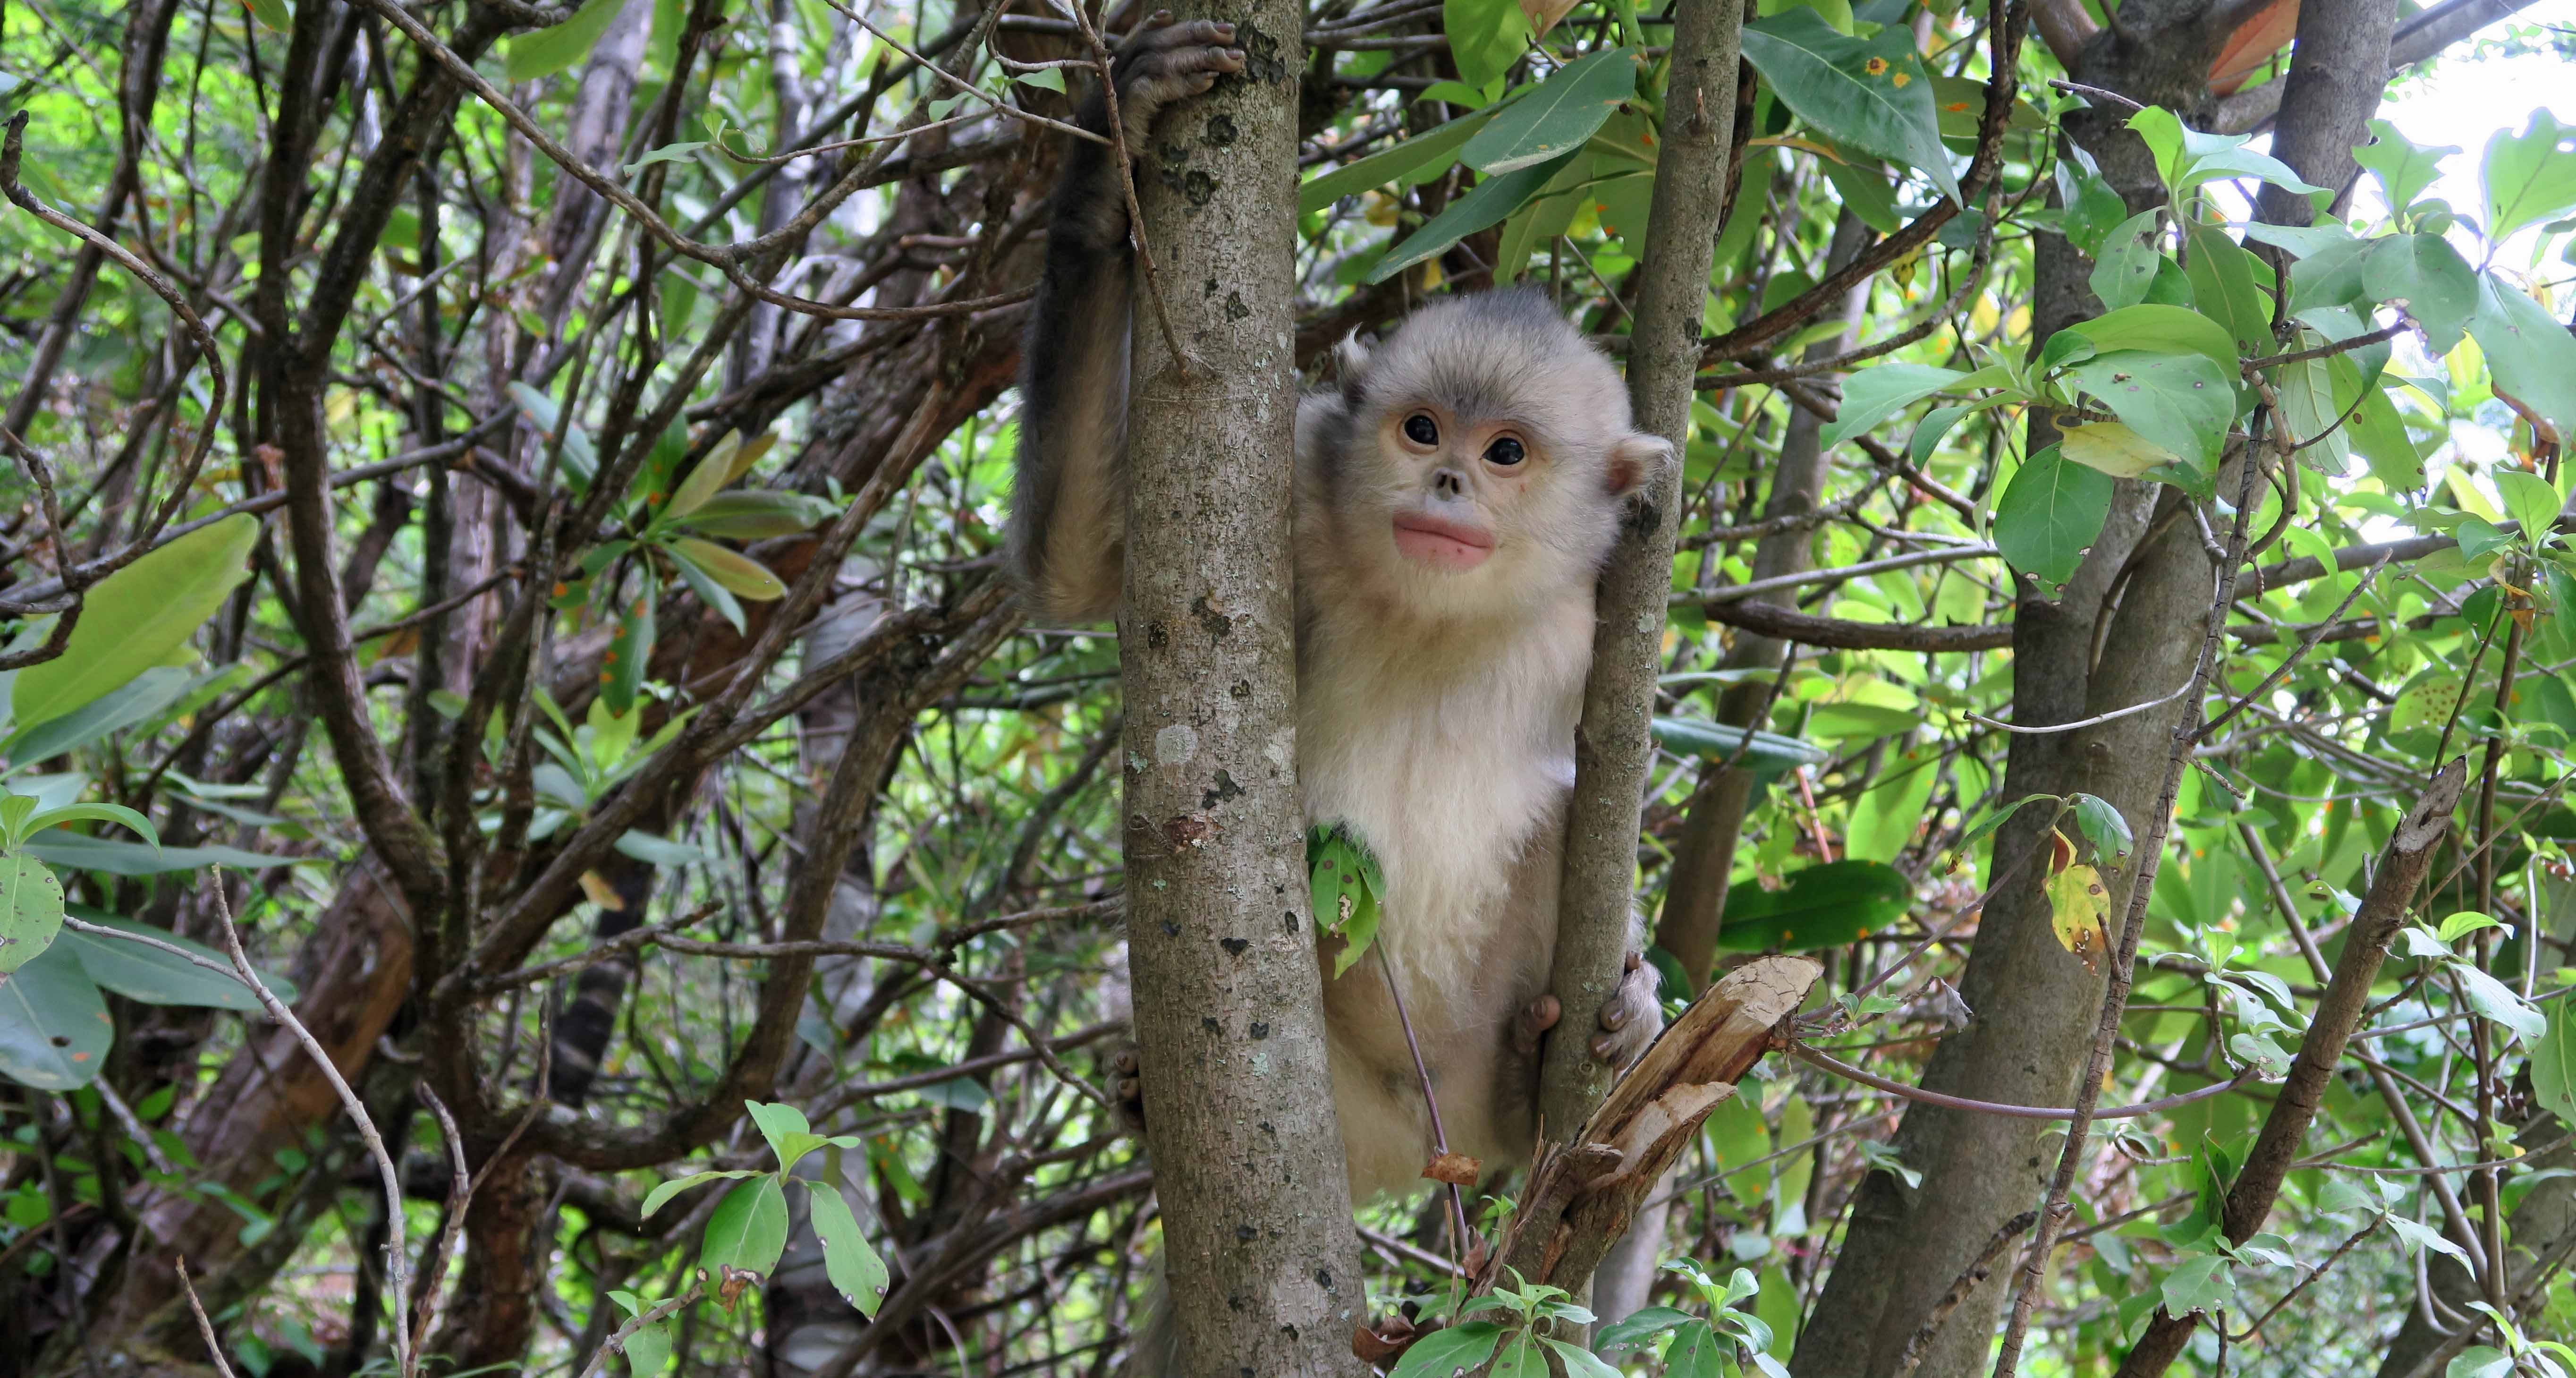
\includegraphics[width=0.8\textwidth]{IMG_1597b}\\[0.5cm]


% Title
\rule{\linewidth}{0.5mm} \\[0.3cm]
{ \huge \bfseries Multi-agent simulation\\with Gama and R \\[0.3cm]
\Large Practical Training Manual}\\[0.3cm]
\rule{\linewidth}{0.5mm} \\[0.5cm]
%\normalsize Website: \url{http://moodle.univ-fcomte.fr/course/view.php?id=8811}


% Author
\noindent

\large Patrick \textsc{Giraudoux} and  Nicolas \textsc{Marilleau}\\[0.5cm]


\includegraphics[width=0.8\textwidth]{Logos}\\[0.5cm]

\vfill

% Bottom of the page
{\small Version of \today, \currenttime}


\end{center}
\end{titlepage}

%%%%%%%%%%%%%%%%%%%%%%%%%%%%%
%%% Non-significant pages %%%
%%%%%%%%%%%%%%%%%%%%%%%%%%%%%

\frontmatter


\clearpage




\vspace*{\fill}

\begin{center}

\includegraphics[width=0.7\textwidth]{LogoSoftwares}
\vskip 0.5 cm
	\color{red}
	\fbox{
		\begin{minipage}{0.7\textwidth}
			\large \textbf{Prerequisite}: to have acquired basic notions in R (e.g. workspace, package,  data.frame, list, for loop, function, etc.) and GIS (e.g. shapefile, attribute table, etc.) and corresponding skills.
		\end{minipage}
	}
\end{center}
\vfill

\tableofcontents


%%%%%%%%%%%%%%%%%%%%%%%%%%%%%%%%%%%%%%%%%%%%
%%% Content of the report and references %%%
%%%%%%%%%%%%%%%%%%%%%%%%%%%%%%%%%%%%%%%%%%%%

\mainmatter
\pagestyle{fancy}

\cleardoublepage

\chapter{Model presentation}
\label{chap:Model Presentation}


\section{Ecological bases}

This model has been inspired by earlier works carried out by \href{https://gdri-ehede.univ-fcomte.fr}{GDRI EHEDE} researchers \citep{Li2015,Clauzel2015,Li2017}.

In brief, after \citet{Li2015}, the black-and-white snub-nosed monkey \textit{Rhinopithecus bieti} is endemic to Yunnan and Tibet, China, and categorized as "endangered" in the IUCN Red List. Surveys have shown that the monkeys live in 15 isolated groups, 12 of them in Yunnan, in a narrow range of the Three Parallel Rivers region, one of the most ecologically important areas of China, the rugged terrain of which makes it difficult to carry out surveys. The species is threatened by habitat alteration, poaching and economic activities such as farming and collection of timber. The areas between populations are damaged by logging, grazing, mining, agriculture and firewood collection. Because of this habitat fragmentation the monkeys may incur a high energy cost if they travel long distances between habitat patches. Fragmentation may subsequently prevent genetic exchange between populations, making the species more vulnerable to extinction. Where required, reserve managers need to establish habitat corridors to facilitate exchange between populations, identifying priority areas for restoration to increase landscape connectivity.

"Snubbies" is a nickname given to the species.

\section{Geography and data}

 Tab.~\ref{tab:habitats} describes the 5 habitat types defined by \citet{Li2017} and fig.~\ref{fig:studyarea} shows the study area and the location of the monkey groups with their ID number.
 
 The shapefile \texttt{source2P} corresponds to this map, and the predefined style file \texttt{source2P.qml} can be used in QGIS for a better display.
 
 The shapefile \texttt{groups} gives the geographical limit of each monkey group. The group ID number, the name of the area and a population size estimate are given as attributes.
 
 \begin{table}[ht]
 	\centering
 	\caption{Habitat quality and composition after \citet{Li2017}}
 	\label{tab:habitats}
 	\begin{tabular}{lllcc}
 		\hline
 		ID & habitat type & Land cover & Altitude & Cost value \\
 		\hline
 		 1&Optimal & \makecell[l]{Armand pine and hemlock,\\ fir-spruce forest, coniferous \\broad-leaved mixed forest} & 2250-4730 & 1 \\
 		 2&Suboptimal  & \makecell[l]{Sclerophyllous evergreen \\broad-leaved forest,\\ shrub-dominated land} & 1220-5240 & 10 \\
 		 3&Suitable &  \makecell[l]{Cold coniferous forest, sub-alpine\\ meadow, broad-leaved forest} & 1310-4950 & 70 \\
 		 4&Unfavourable  & \makecell[l]{Warm coniferous forest (Yunnan \\pine forest), hot dry savanna, \\sparse shrub grass} & 1200-5490 &90 \\
 		 5&Highly unfavourable  & \makecell[l]{Cropland, settlements, water body,\\ barren land} & 1215-5410 & 100 \\
 		\hline
 	\end{tabular}
 \end{table}
 
 
 \begin{figure}[ht]
 	\centering
 	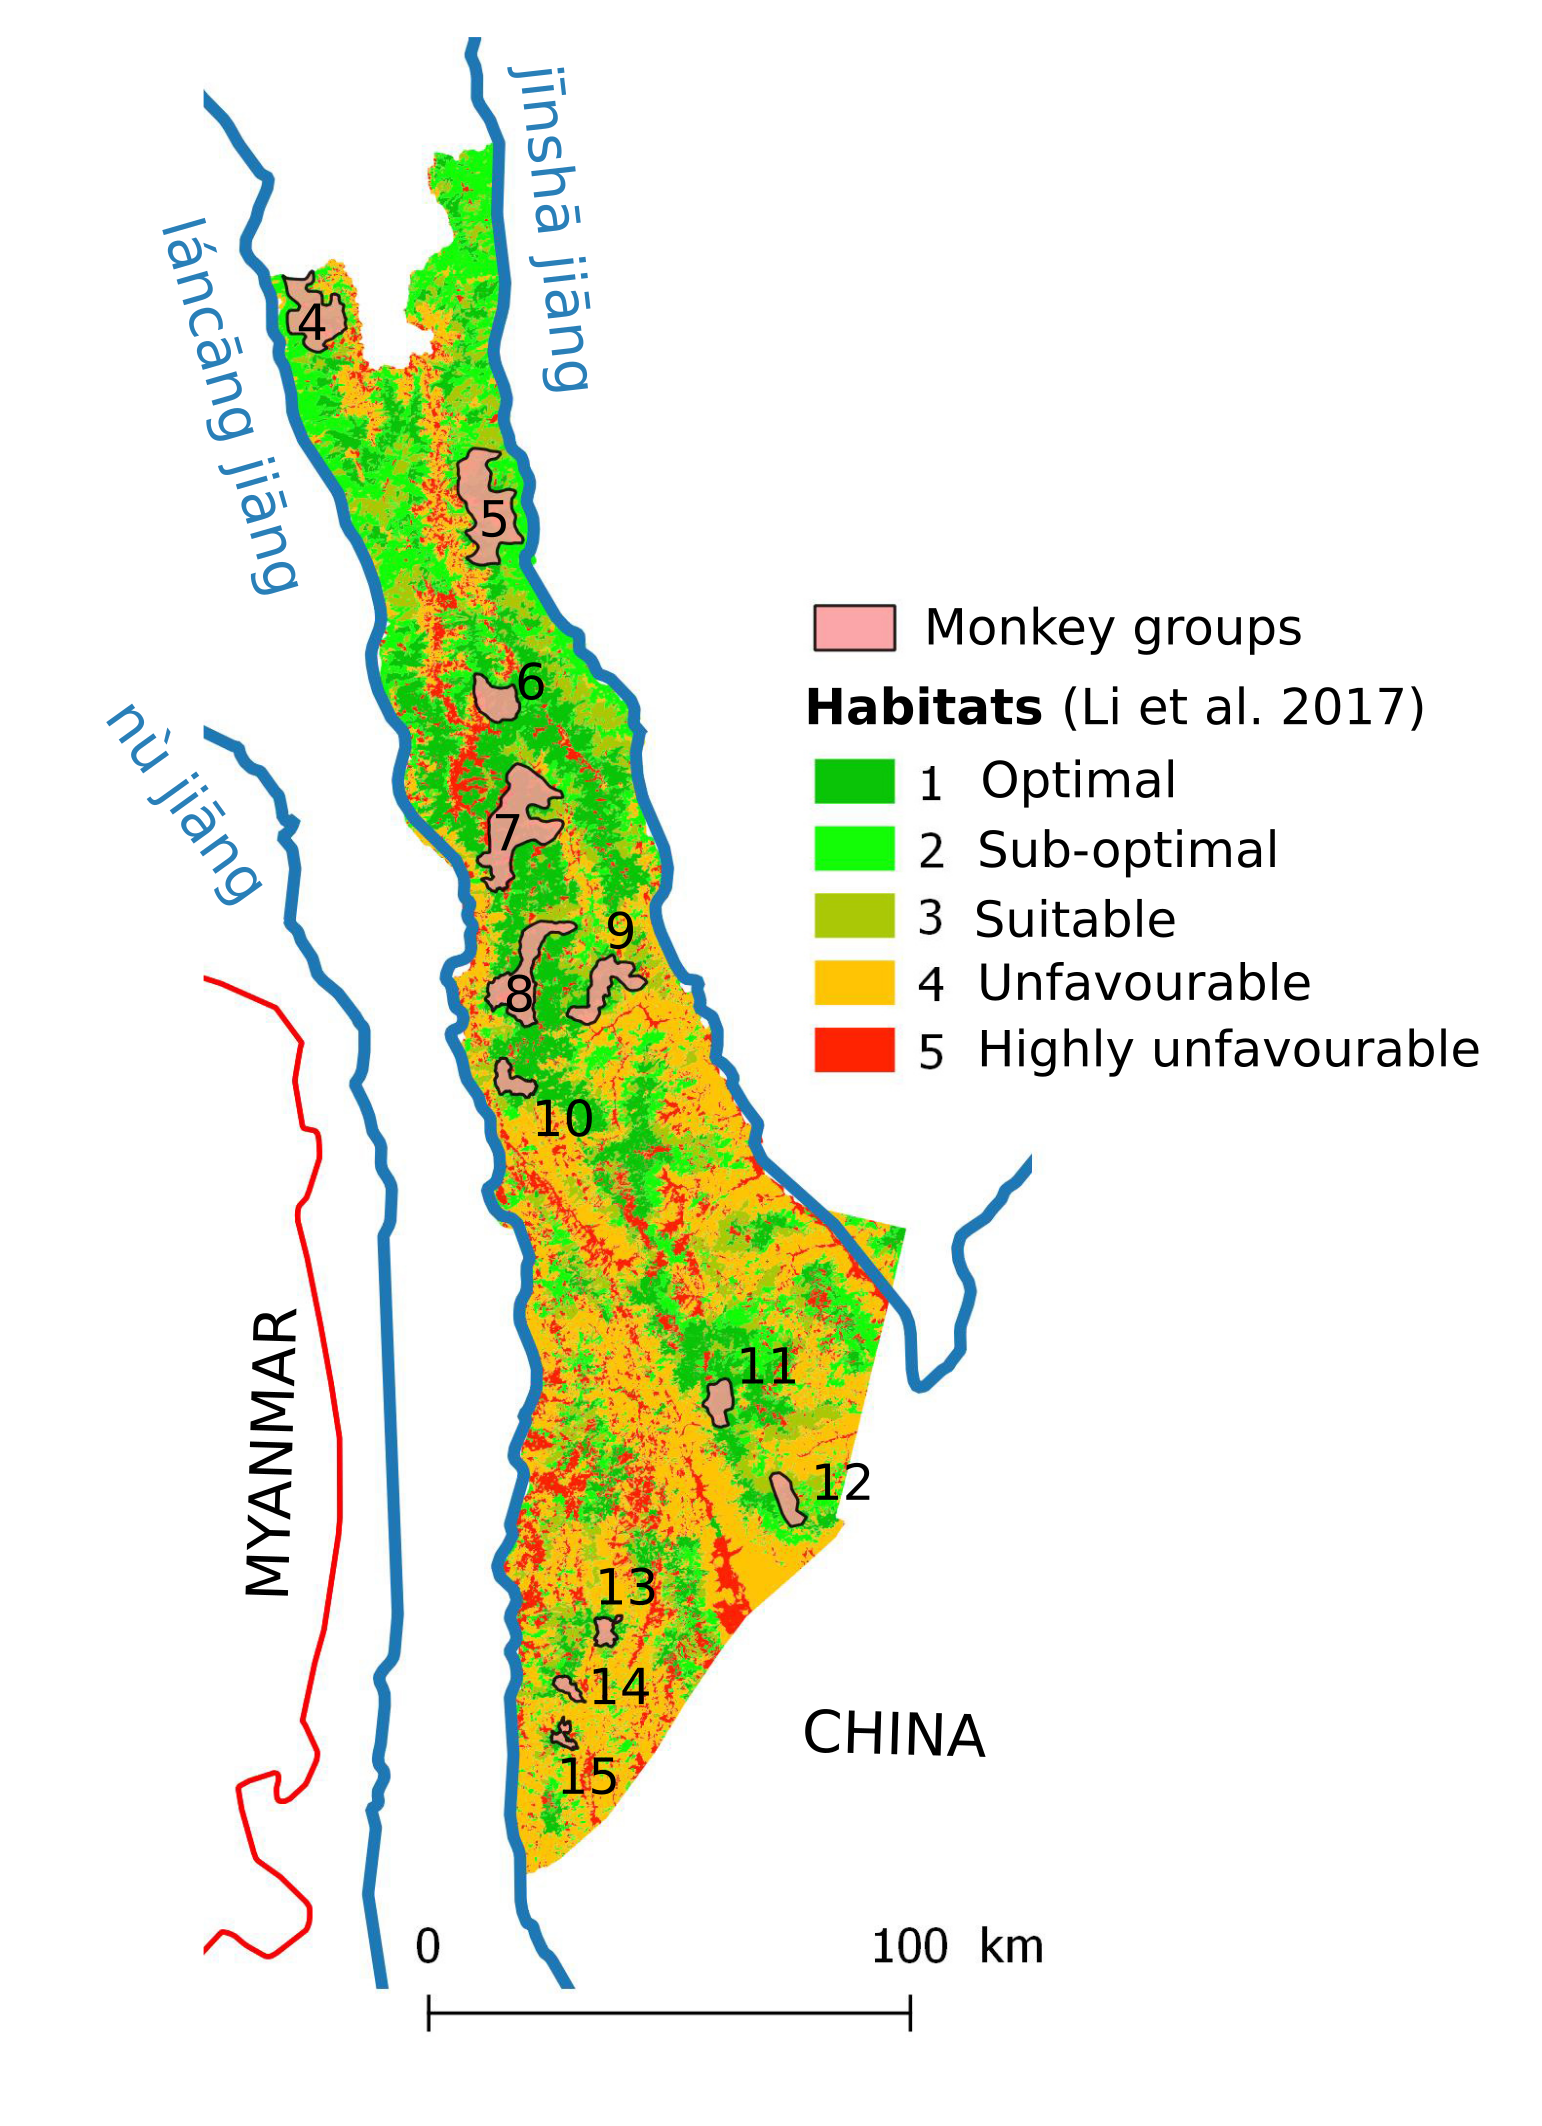
\includegraphics[width=12cm]{Map}
 	\caption{Study area. Numbers on the  map are the group IDs.}
 	\label{fig:studyarea}
 \end{figure}

\section{Model purpose}
Here we want to build a multi-agent model to simulate and explore the effect of habitat and life-history trait 
parameters (real values known or unknown) on snubby dispersion.

\section{Model parameters}

\subsection{Input parameters}
\begin{description}
	\item[step] 1 hour (the iteration time resolution)
	\item[maximum speed] the maximum speed (km/day) that can sustain a snubby in a favourable habitat
	\item[maximum survival]  [0,1] the maximum survival in a favourable habitat. The end user give it per year ($s_y$), but this should be converted to the scale of the step (here hour), using the following formula:
	$s_h=e^{\frac{\ln{s_y}}{365\times24}}$
	\item[disperser proportion] the proportion of snubbies who evade their group and wander outside. The end user give it per year  ($p_y$), but this should be converted to the scale of the step (hour): $p_h=e^{\frac{\ln{p_y}}{365\times24}}$
	\item[habitat viscosity] [0,1] the resistance of a given habitat.  Multiplies the maximum speed to give the speed really sustained in this habitat.
	\item[habitat security] [0,1] the security of a given habitat.  Multiplies the maximum survival to give the actual survival in this habitat.
	\item[habitat dislike] [0,0.5] the probability for a snubby to move into a habitat of lesser quality.
	\item[habitat preference] [0.5,1] the probability for a snubby to move into a habitat of better quality.
	
\end{description}

\subsection{During simulation}
When one snubby dies, one snubby is created in its aboriginal group.


\subsection{Output parameters}

\begin{description}
	\item[Bitmap] Bitmap of snubby distribution (framerate: 6 months).
	\item[Shapefile] Shapefile of snubby distribution with their individual attributes (framerate: 1 year).
	\item[group composition and wanderers] Snubby number in each group and outside, split by group origin.
	
\end{description}






\chapter{Gama model}

\section{Principle}

See:
\begin{itemize}
	\item \citet{Grignard2013}
	\item \url{https://gama-platform.github.io}
	\item \url{https://github.com/gama-platform/gama/wiki/Overview}
	\item \url{https://github.com/gama-platform/gama/wiki}
	\item \url{https://github.com/gama-platform/gama/wiki/Download}
\end{itemize}


\section{Gama in practice}

See practical training on November 6-7, 2018.
\bigskip

\noindent
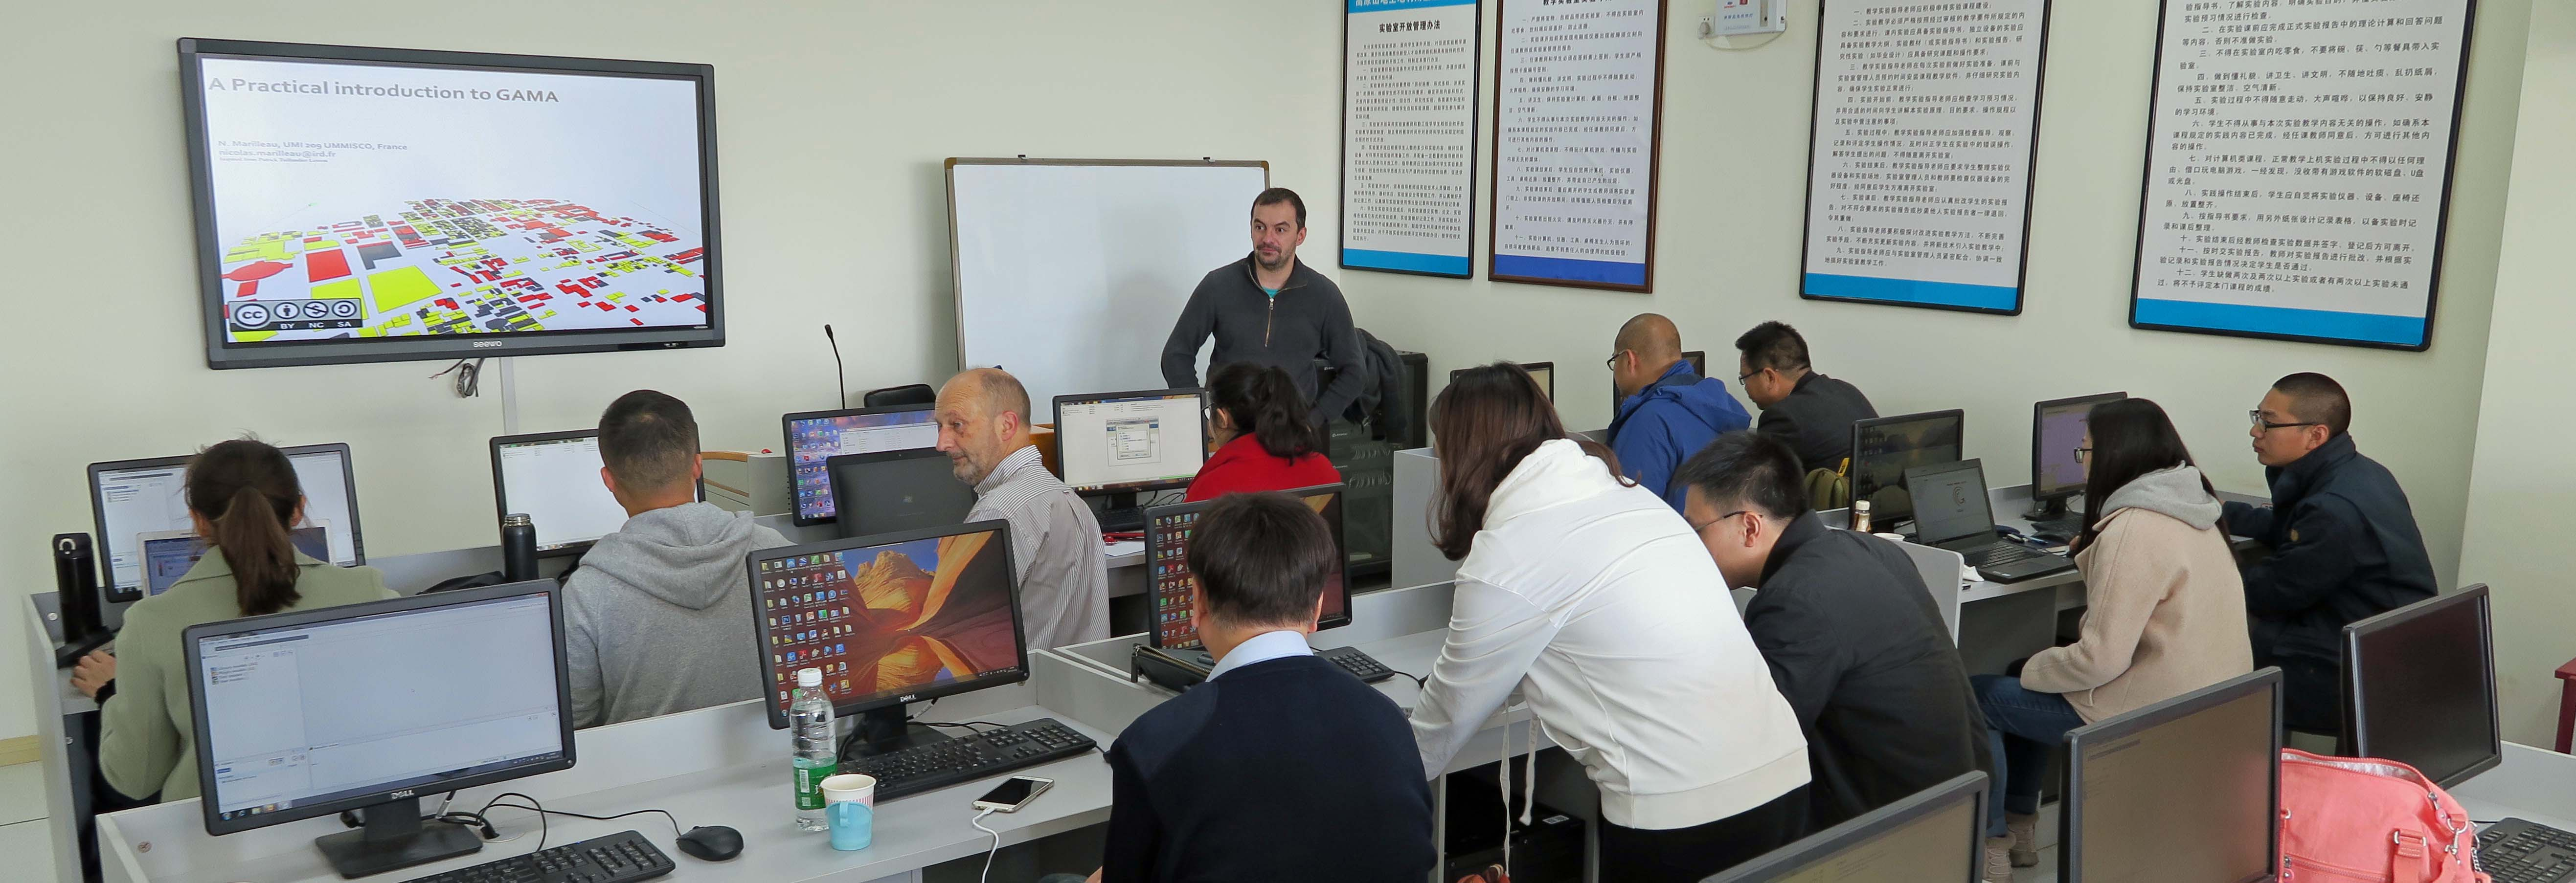
\includegraphics[width=\textwidth]{Classroom}


\chapter{Preparing experiments and analyzing results in R}
\label{chap:Preparing experiments}

Most likely, for full size research, you will carry out simulations on intensive computing systems with hundreds of cores available  in parallel, to run thousands of experiments. Intensive computing systems generally use UNIX and simulations can be run in shell scripts using gama-headless.bat as an entry point. R can be run on such a platform as well and be used for simulations. Here, for teaching purpose, this training manual presents how to do it in R on a personal computer, on a Windows platform. Your computer has likely no more than 2-4 CPU, and it is advisable not to allocate more than two to the job (we will see later how to do it). This means that running a large number of simulations and to simulate on a large number of time steps can be time consuming in this context.

\section{Installing gamar}
\texttt{gamar} is a R package  available at \url{https://github.com/choisy/gamar}. With the \texttt{library(devtools)}, if not already installed, it can be installed on line as following:

\begin{lstlisting}
library(devtools)
devtools::install_github("choisy/gamar")
library(gamar)
\end{lstlisting}

First, one declares the path to the program Gama.exe. Here below an example, but the path you are going to write must be adapted to your own computer:

\begin{lstlisting}
defpath("C:/Program Files/GAMA1.7RC2.Windows.64bits")
\end{lstlisting}

\section{Preparing experiments}


\subsection{Reading the model}

Now, one must read the model (here \texttt{snubbies.gaml}) and extract informations that will be used by R. The path to the model must be declared explicitely (here \texttt{snubbies.gaml}  is in the folder \texttt{"U:/Users/pgiraudo2/gama\_workspace/snubbies/models")}. Again this to adapt to your own computer.

\begin{lstlisting}
experiment1 <- getmodelparameter("U:/Users/pgiraudo2/gama_workspace/snubbies/models/snubbies.gaml","run")
experiment1
\end{lstlisting}


For convenience, we have prepared some home-made functions to ease readings and parameter handling. They are in the file \texttt{HomeFunctions.r}. One sources it, and get a data.frame with attributes:

\label{lab:sourcefunction}
\begin{lstlisting}
source("Homefunctions.r")
ex1<-expe2df(experiment1)
ex1
attributes(ex1)
\end{lstlisting}

\subsection{Preparing the simulations}

The duration of each simulation is stored in a variable, here named \texttt{simulation\_duration} and the number of simulations to run in the variable \texttt{B}

\begin{lstlisting}
simulation_duration <- 5 * 365 * 24 # five years (step is one hour)
B<-10 # number of simulations
\end{lstlisting}

Now, a data.frame must be prepared with the parameter values of each simulation on each row. Note that parameters can be explored randomly allocating values between limits. See for instance the function \texttt{runif} in R (but many others are available).

\begin{lstlisting}
?runif
\end{lstlisting}

Values can be defined quite flexibly and the value(s) of a given parameter can be used as a function of another. See example below.

\label{lab:simuls}
\begin{lstlisting}
simuls<-data.frame(
v_max=0.3472222,
s_max=0.5,
explorer_snubbies=runif(B,0.001,0.1), # random allocation between 0.001 and 0.1 (uniform distribution)
viscosity_factor_habitat_1=runif(B,0.9,1),
viscosity_factor_habitat_2=viscosity_factor_habitat_1*0.9, # the value is defined as a function of another value; here we want viscosity_factor_habitat_2 always be 0.9*viscosity_factor_habitat_1
viscosity_factor_habitat_3=0.5,
viscosity_factor_habitat_4=0.1,
viscosit_factor_habitat_5=0,
security_factor_habitat_1=1,
security_factor_habitat_2=0.9,
security_factor_habitat_3=0.5,
security_factor_habitat_4=0.1,
security_factor_habitat_5=0
)
\end{lstlisting}

Then, experiments can be prepared. This will end up by the creation of one variable \texttt{experimentplan} and as many XML files as experiments (e.g. the number of row of \texttt{simuls}). \textcolor{red}{Pay attention about the unusual way to specify the path with \texttt{setmodelpath}, with a slash "/U:/..." at the beginning. This a provisory way to get around a bug of gama-headless running on Windows}.

\begin{lstlisting}
for (i in 1:nrow(simuls)) {
local_experiment <- experiment1
local_experiment <-  setparametervalue(local_experiment,"max_snubby_speed",simuls[i,"v_max"])
local_experiment <-  setparametervalue(local_experiment,"max_snubby_survival_init",simuls[i,"s_max"])
local_experiment <-  setparametervalue(local_experiment,"explorer_snubbies_init",simuls[i,"explorer_snubbies"])
local_experiment <-  setparametervalue(local_experiment," viscosity_init_habitat_1",simuls[i,"viscosity_factor_habitat_1"])
local_experiment <-  setparametervalue(local_experiment," viscosity_init_habitat_2",simuls[i,"viscosity_factor_habitat_2"])
local_experiment <-  setparametervalue(local_experiment," viscosity_init_habitat_3",simuls[i,"viscosity_factor_habitat_3"])
local_experiment <-  setparametervalue(local_experiment," viscosity_init_habitat_4",simuls[i,"viscosity_factor_habitat_4"])
local_experiment <-  setparametervalue(local_experiment," viscosity_init_habitat_5",simuls[i,"viscosity_factor_habitat_5"])
local_experiment <-  setparametervalue(local_experiment," security_init_habitat_1",simuls[i,"security_factor_habitat_1"])
local_experiment <-  setparametervalue(local_experiment," security_init_habitat_2",simuls[i,"security_factor_habitat_2"])
local_experiment <-  setparametervalue(local_experiment," security_init_habitat_3",simuls[i,"security_factor_habitat_3"])
local_experiment <-  setparametervalue(local_experiment," security_init_habitat_4",simuls[i,"security_factor_habitat_4"])
local_experiment <-  setparametervalue(local_experiment," security_init_habitat_5",simuls[i,"security_factor_habitat_5"])

local_experiment <- setfinalstep(local_experiment,simulation_duration)

local_experiment <- setoutputframerate(local_experiment,"map",10)
local_experiment <- setoutputframerate(local_experiment,"reading_map",10)
local_experiment <- setsimulationid(local_experiment,i)
local_experiment <- setmodelpath(local_experiment,"/U:/Users/pgiraudo2/gama_workspace/snubbies/models/snubbies.gaml")

local_experiment <- setseed(local_experiment,1)

if(i<2)
{

experimentplan <- addtoexperimentplan(simulation = local_experiment)
}
else
{
experimentplan <- addtoexperimentplan(simulation = local_experiment,experimentplan = experimentplan)
}
outFile <- paste0("./input_",formatC(i,width=nchar(nrow(simuls)),flag="0"),".xml")

writemodelparameterfile(experimentplan,outFile)
}

\end{lstlisting}

The  variable of interest is \texttt{experimentplan}. However here, additionally, XML files are saved on the disk with \texttt{writemodelparameterfile}. This can be useful if simulations are run not from R on intensive computing systems and UNIX platforms. There, running simulations with a UNIX shell script is system dependent and will use those XML files (in this case, see with the IT manager how to proceed). Here, with this R script, XML files have been written in the workspace. You can see them either  using Windows Explorer or from R with the following command:

\begin{lstlisting}
dir()
\end{lstlisting}

\section{Running simulations}


Simulations are run very simply then. We add some code lines to get the duration of the simulations at the end.

\begin{lstlisting}
t0<-Sys.time() # store the start time
runexpplan(experimentplan,hpc=2) # run the simulations
t1<-Sys.time() # store the end time
t1-t0
\end{lstlisting}


\section{Reading results}

Simulations results are stored in the folder \texttt{./workgamar}. There one finds:

\begin{itemize}
	\item as many files as experiments, named \texttt{run\_1.xml}, \texttt{run\_2.xml}, etc. Those files just describe the values of the input parameters. No point to read them, all useful information is in the data.frame \texttt{simuls} (see above \ref{lab:simuls}).
	\item a folder named \texttt{out\_run\_1} (or \texttt{out\_run\_2}, \texttt{out\_run\_3}, etc. depending on the number of runs executed before). One finds the following inside:
	\begin{itemize}
		\item a folder named  \texttt{snapshot} containing bitmaps. Note the file name gives the number of the experiment and the step. E.g.\texttt{ reading\_map0-10.png} means experiment \#1 (the experiment numbers are incremented from 0), step 10.
		\item text files \texttt{console-outputs-0.txt}, \texttt{console-outputs-1.txt}, etc. corresponding to the console outputs of experiment \#1, \#2, etc. They are not of much interest when everything goes smoothly, but useful to identify where a simulation has crashed, should it happen.
		\item xml files \texttt{simulation-outputs0.xml}, \texttt{simulation-outputs01.xml}, etc. corresponding to the outputs of experiment \#1, \#2, etc.
	\end{itemize}
\end{itemize}

One needs some R code to read the XML file. Here we use a home-made function \texttt{readNamesXMLOutputs} to read variable names (it as been sourced before see \ref{lab:sourcefunction})

\begin{lstlisting}
library(XML)

path<-paste0("./workgamar/out_run_1/") # the path to the XML files
outs<-dir(path,pattern="*.xml") # one reads them
outs<-outs[order(as.numeric(substr(outs,19,nchar(outs)-4)))] # to get the files in the right order whatever the number of digit

outs<-paste0(path,outs) # now the full path with file names
outs

mycolnames<-readNamesXMLOutputs(outs[1]) # one uses a home made function to extract the variables names from one of the XML files

results<-rep(list(NA),length(outs)) # one prepares an empty list to store the readings
for(i in 1:length(outs)) {
	results[[i]]<-xmlToDataFrame(outs[i])  # we read the XML file into a data.frame
	names(results[[i]])<-mycolnames # one gives names to columns
}

names(results)<-outs # one gives a name to each experiments

results

\end{lstlisting}




\section{Analysing results}

To come soon...

%\appendix

\bibliographystyle{apa-good}
\bibliography{BiblioManual}

\clearpage


\end{document}